\chapter*{chapitre 4}
\markboth{Chapitre 4 }{4 Release 1 : Développement du Backend} %pour afficher l'entete
 \addcontentsline{toc}{chapter}{4 Release 1 : Développement du Backend}

\textbf{\Huge Release 1 : Développement du Backend}

\setcounter{chapter}{4}
\setcounter{section}{0}

\section{Introduction}

La Release 0 a livré les trois briques d'infrastructure fondamentales de la plateforme : cluster Kubernetes isolé par tenant, exécution serverless via Knative Serving et bus d'événements Kafka opéré par Strimzi. La Release 1, objet de ce chapitre, a pour objectif de bâtir, au-dessus de ce socle, le \textbf{backend applicatif} qui transforme ces briques techniques isolées en une plateforme cohérente exploitable par un utilisateur final. Elle regroupe trois sprints : le Sprint 3, qui relie Knative Serving et Kafka au travers de Knative Eventing ; le Sprint 4, qui met en place l'authentification, les rôles et les permissions ; et le Sprint 5, qui livre la première version exploitable de la gestion des applications ainsi que le point de départ du pipeline d'intégration continue du backend. C'est à partir de cette release que les premiers cas d'utilisation accessibles à un acteur humain apparaissent dans le mémoire.


\section{Sprint 3 : Mise en œuvre de Knative Eventing}

\subsection{Introduction}

Ce sprint a pour objectif de relier, côté backend, les deux briques serverless et événementielle mises en place à la Release 0, en implémentant la capacité à connecter un sujet Kafka à une application Knative de sorte qu'un message publié sur ce sujet puisse réveiller automatiquement l'application concernée.

\subsection{Objectifs du Sprint}

\begin{itemize}
    \item Implémenter, côté backend, la création programmatique des ressources Knative Eventing (\texttt{Broker}, \texttt{Trigger}, \texttt{KafkaSource}) nécessaires pour relier un sujet Kafka à un service Knative.
    \item Garantir la cohérence entre l'état stocké en base de données et l'état réel des ressources créées sur le cluster.
    \item Permettre la suppression propre des ressources d'Eventing lorsqu'une application est supprimée, afin d'éviter les ressources orphelines.
\end{itemize}

\subsection{Sprint Backlog}

\begin{table}[!ht]
\begin{center}
     \begin{tabular}{|l{11cm}|l{3cm}|}
     \hline
     \textbf{User Story} & \textbf{Statut} \\
     \hline
     En tant que développeur backend, je veux créer une ressource KafkaSource associée à une application & Réalisé \\
     \hline
     En tant que développeur backend, je veux créer un Trigger reliant un Broker à une application & Réalisé \\
     \hline
     En tant qu'exploitant, je veux que la suppression d'une application supprime aussi ses ressources d'Eventing & Réalisé \\
     \hline
     En tant qu'exploitant, je veux que l'état en base reste cohérent avec l'état réel du cluster & Réalisé (après corrections) \\
     \hline
     \end{tabular}
     \caption{Sprint Backlog — Sprint 3}
     \label{tab:sb-sprint3}
     \end{center}
\end{table}

\subsection{Présentation des composants développés}

Ce sprint introduit la classe \texttt{EventingService} du backend (module \texttt{eventing}), qui encapsule la création, la lecture et la suppression des ressources Knative Eventing via l'API générique de Fabric8, selon le même principe que celui déjà retenu pour Knative Serving et Kafka. Une ressource \texttt{Broker} unique est utilisée par espace de noms tenant ; chaque association entre un sujet Kafka et une application se traduit par la création d'une ressource \texttt{KafkaSource} (qui consomme le sujet et transmet les messages au \textit{Broker} sous forme de \textit{CloudEvents}) et d'une ressource \texttt{Trigger} (qui filtre les événements du \textit{Broker} selon leur type et les route vers l'URL du service Knative cible).

\subsection{Description du cas d'utilisation « Configurer un déclencheur d'événement »}

\subsubsection{Description textuelle}

\begin{table}[!ht]
\begin{center}
     \begin{tabular}{|l{3.5cm}|p{9cm}|}
     \hline
     \textbf{Nom} & Configurer un déclencheur d'événement \\
     \hline
     \textbf{Acteur} & CLIENT\_ADMIN, MEMBER (avec permission de gestion de l'Eventing) \\
     \hline
     \textbf{Pré-condition} & L'application cible est déployée ; le sujet Kafka source existe \\
     \hline
     \textbf{Scénario nominal} & 1. L'utilisateur sélectionne un sujet Kafka et une application cible. 2. Le backend crée la ressource \texttt{KafkaSource} rattachée au sujet. 3. Le backend crée la ressource \texttt{Trigger} associée, filtrant sur le type d'événement et pointant vers l'URL du service Knative de l'application. 4. La configuration est persistée et son état est renvoyé à l'utilisateur. \\
     \hline
     \textbf{Post-condition} & Toute publication ultérieure sur le sujet Kafka déclenche, le cas échéant, le réveil et l'invocation de l'application. \\
     \hline
     \end{tabular}
     \caption{Description textuelle du cas d'utilisation « Configurer un déclencheur d'événement »}
     \label{tab:uc-eventing}
     \end{center}
\end{table}

\subsubsection{Diagramme de séquence}

\begin{figure}[h!]
 \centering
    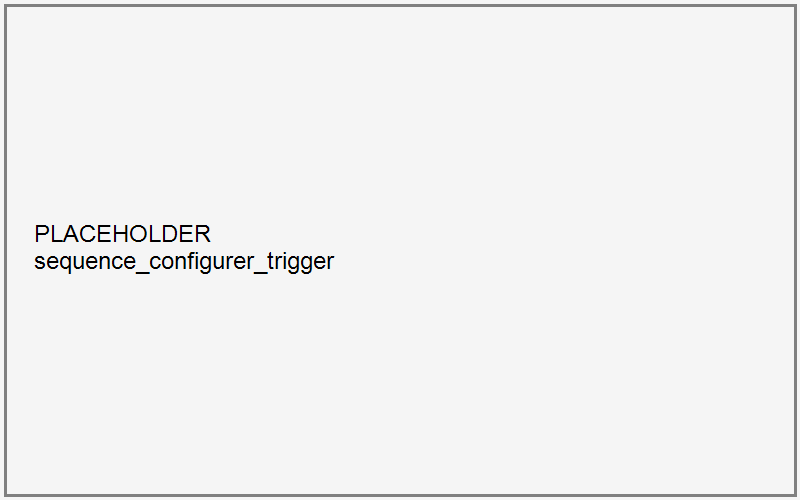
\includegraphics[width=15cm]{diagrammes/sequence_configurer_trigger.png}
    \caption{Diagramme de séquence — Configuration d'un déclencheur d'événement}
    \label{fig:seq-trigger}
\end{figure}

\subsection{Réalisation}

La création d'un déclencheur suit la logique suivante côté backend : validation de la propriété de l'application et du sujet Kafka par l'utilisateur courant (au travers de \texttt{UserContextService}), construction du manifeste \texttt{KafkaSource} référençant le sujet et le \textit{Broker} du tenant, construction du manifeste \texttt{Trigger} référençant le \textit{Broker} et l'URL interne du service Knative cible, puis application séquentielle de ces deux ressources sur le cluster.

\subsection{Difficultés rencontrées et solutions apportées}

L'implémentation initiale de ce module a présenté plusieurs anomalies de cohérence entre la base de données et l'état réel du cluster, mises en évidence lors d'un audit dédié du module Eventing/Kafka :

\begin{itemize}
    \item \textbf{Exceptions Fabric8 silencieusement absorbées} : certains appels de création de ressources capturaient les exceptions sans les propager ni les journaliser, laissant croire à un succès alors que la ressource n'avait pas été créée sur le cluster. \textit{Solution} : propagation et journalisation systématiques des erreurs Fabric8, avec échec explicite de l'opération côté API.
    \item \textbf{Espace de noms codé en dur} : certaines opérations référençaient un espace de noms fixe au lieu de celui du tenant courant. \textit{Solution} : résolution systématique de l'espace de noms à partir du contexte du tenant.
    \item \textbf{Ressources \texttt{Trigger} orphelines à la suppression} : la suppression d'une application ne supprimait pas systématiquement le \texttt{Trigger} associé, laissant une ressource orpheline sur le cluster. \textit{Solution} : suppression en cascade du \texttt{Trigger} et du \texttt{KafkaSource} lors de la suppression logique d'une application.
    \item \textbf{État de disponibilité non resynchronisé} : le statut de disponibilité d'un déclencheur n'était pas remis à jour après une reconfiguration. \textit{Solution} : resynchronisation explicite de l'état après chaque opération de création/mise à jour.
\end{itemize}

\subsection{Résultat obtenu}

Au terme de ce sprint, un client peut, en théorie via l'API backend, relier un sujet Kafka à l'une de ses applications de sorte que celle-ci soit automatiquement réveillée à la réception d'un message. Cette fonctionnalité ne sera exposée dans l'interface graphique du portail qu'à partir du Sprint 8 ; jusque-là, elle est validée par des appels directs à l'API (voir chapitre de validation).

\subsection{Conclusion du Sprint}

Ce sprint a permis de relier effectivement les deux briques serverless et événementielle du système, en identifiant et corrigeant plusieurs anomalies de cohérence critiques pour la fiabilité de la plateforme. Le sprint suivant s'attache désormais à sécuriser l'accès à l'ensemble de ces fonctionnalités.


\section{Sprint 4 : Authentification et sécurité}

\subsection{Introduction}

Ce sprint a pour objectif de mettre en place le mécanisme d'authentification et de contrôle d'accès de la plateforme, préalable indispensable avant d'exposer la moindre fonctionnalité applicative à un utilisateur final.

\subsection{Objectifs du Sprint}

\begin{itemize}
    \item Intégrer Keycloak comme fournisseur d'identité (OpenID Connect / OAuth2) pour l'authentification des utilisateurs.
    \item Définir le modèle de rôles (ADMIN, CLIENT\_ADMIN, MEMBER) et de permissions granulaires pour les MEMBER.
    \item Sécuriser l'API REST du backend en tant que serveur de ressources OAuth2 (validation des jetons JWT).
    \item Mettre en place un mécanisme d'authentification alternatif par clé d'API, destiné aux usages machine-à-machine (pipelines CI/CD).
    \item Mettre en place la synchronisation entre l'utilisateur authentifié auprès de Keycloak et l'entité utilisateur locale du backend.
\end{itemize}

\subsection{Sprint Backlog}

\begin{table}[!ht]
\begin{center}
     \begin{tabular}{|l{11cm}|l{3cm}|}
     \hline
     \textbf{User Story} & \textbf{Statut} \\
     \hline
     En tant qu'utilisateur, je veux me connecter à la plateforme avec mon compte & Réalisé \\
     \hline
     En tant que CLIENT\_ADMIN, je veux inviter des membres et leur attribuer des permissions & Réalisé \\
     \hline
     En tant que backend, je veux valider les jetons émis par Keycloak sur chaque requête & Réalisé \\
     \hline
     En tant que CLIENT\_ADMIN, je veux générer une clé d'API pour mon pipeline CI/CD & Réalisé \\
     \hline
     \end{tabular}
     \caption{Sprint Backlog — Sprint 4}
     \label{tab:sb-sprint4}
     \end{center}
\end{table}

\subsection{Diagramme de cas d'utilisation du Sprint}

\begin{figure}[h!]
 \centering
    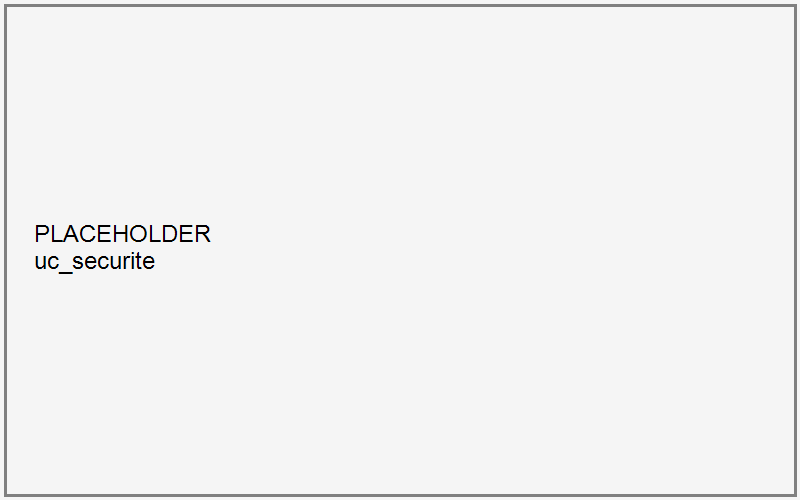
\includegraphics[width=12cm]{diagrammes/uc_securite.png}
    \caption{Diagramme de cas d'utilisation — Authentification et sécurité}
    \label{fig:uc-securite}
\end{figure}

\subsection{Présentation des composants développés}

\begin{itemize}
    \item \texttt{KeycloakJwtAuthConverter} : convertit les jetons JWT émis par Keycloak en objets d'authentification Spring Security, en extrayant les rôles applicatifs à partir de la revendication (\textit{claim}) \texttt{realm\_access.roles} du jeton.
    \item \texttt{UserSyncFilter} : filtre de sécurité créant, si nécessaire, l'entité \texttt{User} locale correspondant à l'utilisateur authentifié auprès de Keycloak lors de sa première requête, assurant la cohérence entre l'identité fédérée et le modèle de données interne.
    \item \texttt{UserRole} (énumération \texttt{ADMIN}, \texttt{CLIENT\_ADMIN}, \texttt{MEMBER}) et \texttt{Permission} : modèle de rôles et de permissions granulaires (déploiement, suppression d'application, gestion Kafka, gestion Eventing, consultation des journaux, consultation de la supervision, consultation et export de la facturation), vérifiées par le \texttt{PermissionService}.
    \item \texttt{UserContextService} : résout systématiquement l'identité \og effective \fg{} d'un appelant, en rattachant un \texttt{MEMBER} au compte de son \texttt{CLIENT\_ADMIN} pour toute opération portant sur la propriété d'une ressource.
    \item \texttt{ApiKeyService} / \texttt{ApiKeyFilter} : génération de clés d'API au format \texttt{plat\_<chaîne aléatoire>}, dont seul le hachage SHA-256 et un préfixe de 12 caractères sont conservés en base ; filtre de sécurité validant ces clés en amont de la chaîne Spring Security standard, pour un usage machine-à-machine (pipelines CI/CD).
\end{itemize}

\subsection{Description du cas d'utilisation « Se connecter à la plateforme »}

\subsubsection{Description textuelle}

\begin{table}[!ht]
\begin{center}
     \begin{tabular}{|l{3.5cm}|p{9cm}|}
     \hline
     \textbf{Nom} & Se connecter à la plateforme \\
     \hline
     \textbf{Acteur} & CLIENT\_ADMIN, MEMBER, ADMIN \\
     \hline
     \textbf{Pré-condition} & L'utilisateur possède un compte enregistré dans le royaume (\textit{realm}) Keycloak de la plateforme \\
     \hline
     \textbf{Scénario nominal} & 1. L'utilisateur saisit ses identifiants sur le portail. 2. Le portail échange ces identifiants contre un jeton JWT auprès de Keycloak. 3. Le portail joint ce jeton à chacune de ses requêtes vers le backend. 4. Le backend valide la signature et la validité du jeton, en extrait les rôles, et synchronise l'utilisateur local si besoin. 5. L'utilisateur accède aux fonctionnalités autorisées par son rôle et ses permissions. \\
     \hline
     \textbf{Post-condition} & Une session applicative authentifiée est établie côté portail. \\
     \hline
     \end{tabular}
     \caption{Description textuelle du cas d'utilisation « Se connecter à la plateforme »}
     \label{tab:uc-login}
     \end{center}
\end{table}

\subsubsection{Diagramme de séquence}

\begin{figure}[h!]
 \centering
    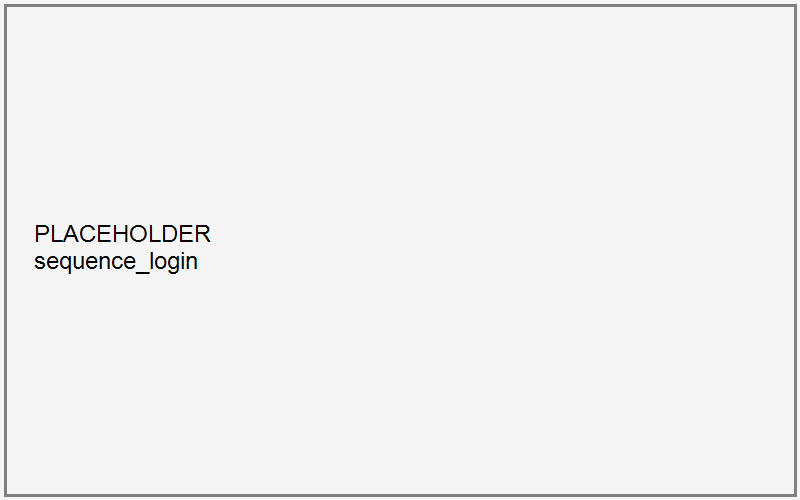
\includegraphics[width=15cm]{diagrammes/sequence_login.png}
    \caption{Diagramme de séquence — Authentification d'un utilisateur}
    \label{fig:seq-login}
\end{figure}

\subsection{Difficultés rencontrées et solutions apportées}

\begin{itemize}
    \item \textbf{Flux d'authentification implémenté côté portail} : l'échange des identifiants contre un jeton a été implémenté côté frontend selon le flux \textit{Resource Owner Password Credentials} (envoi direct du couple identifiant/mot de passe à Keycloak), plutôt que le flux \textit{Authorization Code avec PKCE}, recommandé pour les applications monopages car il évite toute manipulation du mot de passe par le code applicatif. Ce point a été identifié lors de l'audit de sécurité de la plateforme et \textbf{assumé comme un risque produit accepté} plutôt que corrigé dans le délai du projet ; il est repris explicitement dans les limites du chapitre de validation.
    \item \textbf{Jeton exposé dans les paramètres d'URL du flux de journaux en temps réel (SSE)} : le mécanisme natif \texttt{EventSource} du navigateur ne permettant pas l'envoi d'en-têtes HTTP personnalisés, le jeton d'authentification était initialement transmis en paramètre d'URL, avec un risque de fuite dans les journaux d'infrastructure (proxy, ingress). \textit{Solution} : migration vers la bibliothèque \texttt{@microsoft/fetch-event-source}, qui permet l'envoi du jeton dans l'en-tête \texttt{Authorization} standard, avec conservation d'un filtre de secours (\texttt{SseTokenFilter}) pour compatibilité.
    \item \textbf{Rôles Kubernetes (RBAC) sous-déclarés} : le rôle attribué au compte de service du backend ne couvrait pas initialement l'ensemble des ressources réellement manipulées (Knative, Eventing, Strimzi). \textit{Solution} : reconstruction du \texttt{ClusterRole} à partir des permissions effectivement nécessaires, vérifiées par la commande \texttt{kubectl auth can-i}.
\end{itemize}

\subsection{Résultat obtenu}

À l'issue de ce sprint, l'ensemble des fonctionnalités développées lors des sprints précédents et suivants sont protégées par une authentification centralisée via Keycloak, un modèle de rôles à trois niveaux et un système de permissions granulaires pour les membres d'équipe, ainsi qu'un mécanisme d'authentification alternatif par clé d'API pour les usages automatisés.

\subsection{Conclusion du Sprint}

Ce sprint a doté la plateforme d'un socle de sécurité indispensable avant l'ouverture de ses fonctionnalités métier à des utilisateurs réels. Le sprint suivant s'appuie directement sur ce socle pour livrer la première version exploitable de la gestion des applications.


\section{Sprint 5 : Gestion des applications et début du pipeline CI/CD Backend}

\subsection{Introduction}

Ce sprint constitue un jalon majeur du projet : il livre la première fonctionnalité complète et bout-en-bout accessible à un client de la plateforme — le déploiement d'une application — en s'appuyant sur l'ensemble des briques développées lors des sprints précédents (Knative Serving, authentification, permissions). Il initie en parallèle l'automatisation de la construction et du déploiement du backend lui-même.

\subsection{Objectifs du Sprint}

\begin{itemize}
    \item Développer le cycle de vie complet de gestion d'une application cliente : création, consultation, mise à jour, suppression logique, historique de révisions et retour à une révision antérieure.
    \item Garantir la réactivité de l'API en rendant le déploiement effectif sur le cluster asynchrone par rapport à la requête HTTP du client.
    \item Synchroniser en continu le statut de l'application en base de données avec son état réel sur le cluster.
    \item Mettre en place un premier pipeline Jenkins pour la construction, la publication et le déploiement automatisés du backend, en utilisant Kaniko pour la construction de l'image sans démon Docker privilégié.
\end{itemize}

\subsection{Sprint Backlog}

\begin{table}[!ht]
\begin{center}
     \begin{tabular}{|l{11cm}|l{3cm}|}
     \hline
     \textbf{User Story} & \textbf{Statut} \\
     \hline
     En tant que client, je veux déployer une application à partir d'une image Docker & Réalisé \\
     \hline
     En tant que client, je veux consulter l'état de mes applications en temps réel & Réalisé \\
     \hline
     En tant que client, je veux mettre à jour ou supprimer une application & Réalisé \\
     \hline
     En tant que client, je veux consulter l'historique des révisions et revenir à une version antérieure & Réalisé \\
     \hline
     En tant qu'exploitant, je veux que le backend soit reconstruit et redéployé automatiquement à chaque évolution du code & Réalisé \\
     \hline
     \end{tabular}
     \caption{Sprint Backlog — Sprint 5}
     \label{tab:sb-sprint5}
     \end{center}
\end{table}

\subsection{Diagramme de cas d'utilisation du Sprint}

\begin{figure}[h!]
 \centering
    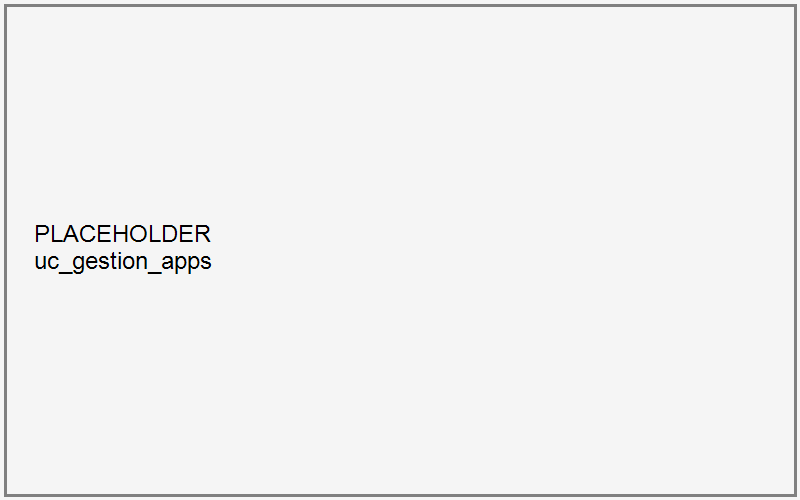
\includegraphics[width=12cm]{diagrammes/uc_gestion_apps.png}
    \caption{Diagramme de cas d'utilisation — Gestion des applications}
    \label{fig:uc-apps}
\end{figure}

\subsection{Présentation des composants développés}

\begin{itemize}
    \item \texttt{App} : entité métier représentant une application déployée, avec son statut (\texttt{DEPLOYING}, \texttt{RUNNING}, \texttt{FAILED}, \texttt{DELETED}, etc.), son image, son port et ses paramètres de mise à l'échelle.
    \item \texttt{AppController} / \texttt{AppService} : exposition de l'API REST de gestion des applications et implémentation de la logique métier (génération d'un nom de service unique compatible DNS, délégation de propriété MEMBER $\rightarrow$ CLIENT\_ADMIN).
    \item \texttt{AppDeploymentAsyncRunner} : composant dédié à l'exécution asynchrone du déploiement effectif sur le cluster, découplée du cycle de la requête HTTP entrante.
    \item \texttt{KnativeWatcher} : observateur Fabric8 surveillant en continu l'état des ressources Knative du cluster et répercutant les changements de statut sur l'entité \texttt{App} correspondante en base de données.
    \item \texttt{DeploymentLog} et \texttt{LogSseService} : journalisation des événements de cycle de vie d'une application et diffusion en temps réel au portail via un flux d'événements serveur (SSE).
\end{itemize}

\subsection{Description du cas d'utilisation « Déployer une application »}

\subsubsection{Description textuelle}

\begin{table}[!ht]
\begin{center}
     \begin{tabular}{|l{3.5cm}|p{9cm}|}
     \hline
     \textbf{Nom} & Déployer une application \\
     \hline
     \textbf{Acteur} & CLIENT\_ADMIN, MEMBER (avec permission de déploiement) \\
     \hline
     \textbf{Pré-condition} & L'utilisateur est authentifié et dispose de la permission \texttt{DEPLOY\_APP} \\
     \hline
     \textbf{Scénario nominal} & 1. L'utilisateur renseigne le formulaire de déploiement (nom, image, port, ressources, bornes de mise à l'échelle) et génère un nom de service unique. 2. L'entité \texttt{App} est créée avec le statut \texttt{DEPLOYING} et un \texttt{DeploymentLog} est émis. 3. Le backend répond immédiatement, puis déclenche de manière asynchrone la création de la ressource Knative correspondante. 4. Le statut de l'application est mis à jour en temps réel à mesure que Knative provisionne le service. \\
     \hline
     \textbf{Scénario étendu} & Si l'utilisateur a activé l'onglet « Kafka Trigger » du formulaire (sujet Kafka + éventuel type de filtre), et une fois le déploiement Knative réussi, le backend crée automatiquement, dans la même exécution asynchrone, un \texttt{KafkaSource} et un \texttt{Trigger} pointant vers l'URL du service qui vient d'être déployé — sans étape manuelle supplémentaire de l'utilisateur. \\
     \hline
     \textbf{Post-condition} & L'application est déployée et accessible (et, le cas échéant, câblée à son sujet Kafka), ou son statut reflète l'échec du déploiement. \\
     \hline
     \end{tabular}
     \caption{Description textuelle du cas d'utilisation « Déployer une application »}
     \label{tab:uc-deploy}
     \end{center}
\end{table}

\subsubsection{Diagramme de séquence}

Le diagramme de séquence détaillé de ce cas d'utilisation reprend et détaille, au niveau des classes du backend introduites dans ce sprint, le processus déjà présenté de manière transverse à la figure~\ref{fig:seq-deploiement} du chapitre 2 (Analyse et spécification des besoins).

\begin{figure}[h!]
 \centering
    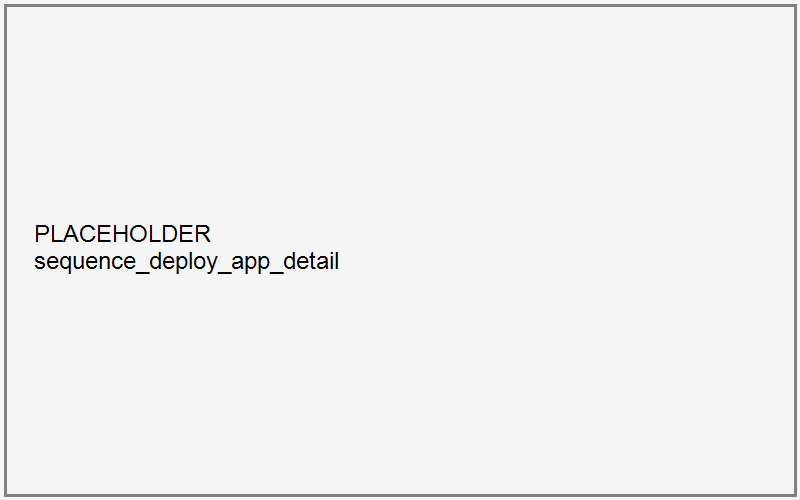
\includegraphics[width=15.5cm,height=21cm]{diagrammes/sequence_deploy_app_detail.png}
    \caption{Diagramme de séquence détaillé — Déployer une application}
    \label{fig:seq-deploy-detail}
\end{figure}

\subsection{Présentation de la réalisation}

Le formulaire de déploiement et la vue de détail d'une application (statut en temps réel, journaux, historique de révisions) sont accessibles depuis le portail client à partir du Sprint 8, lorsque l'interface graphique correspondante est livrée. À ce stade du projet (fin de Sprint 5), ces fonctionnalités ont été validées par des appels directs à l'API REST (voir captures d'écran de tests API au chapitre de validation).

\subsubsection{Intégration Kafka automatique au moment du déploiement}

Au-delà du scénario nominal, \texttt{AppDeploymentAsyncRunner} implémente un second chemin, optionnel, qui anticipe sur la fonctionnalité développée au Sprint 6 : si la requête de déploiement porte un indicateur \texttt{kafkaEnabled} et l'identifiant d'un sujet Kafka existant, le backend crée automatiquement, \textbf{juste après le succès du déploiement Knative et dans la même exécution asynchrone}, un \texttt{KafkaSource} puis un \texttt{Trigger} pointant vers l'URL du service qui vient d'être déployé. Ce chemin se distingue du flux manuel de configuration d'un déclencheur présenté au Sprint 6 sur un point technique important : l'URL transmise en paramètre \texttt{action} au \texttt{Trigger} est ici directement celle que \texttt{KnativeService.deploy()} vient de renvoyer pour l'application en cours de création — l'égalité entre le nom d'abonné du \texttt{Trigger} et le service réellement déployé est donc garantie par construction, alors qu'elle dépend, dans le flux manuel du Sprint 6, de la valeur fournie librement par l'appelant. En cas d'échec du déploiement Knative, cette étape n'est jamais exécutée : aucune ressource d'Eventing n'est créée pour une application qui n'a pas démarré.

\subsection{Le pipeline CI/CD Backend}

Un premier pipeline Jenkins est mis en place pour le backend, structuré selon les étapes suivantes : récupération du code source (avec réessai automatique en cas d'échec transitoire), compilation Maven (\texttt{mvn clean package}), construction de l'image de conteneur par \textbf{Kaniko} — outil permettant de construire une image Docker à l'intérieur même du pod Jenkins, sans nécessiter de démon Docker privilégié — publication de l'image sur Docker Hub, puis mise à jour de l'image du déploiement Kubernetes du backend (\texttt{kubectl set image}) suivie de la vérification du succès du déploiement (\texttt{kubectl rollout status}).

\subsection{Difficultés rencontrées et solutions apportées}

\begin{itemize}
    \item \textbf{Déploiement \og asynchrone \fg{} en réalité bloquant} : la méthode de création d'une application invoquait sa méthode de déploiement asynchrone directement sur \texttt{this}, contournant ainsi le mécanisme de proxy AOP de Spring responsable de l'exécution effective en tâche de fond. La requête HTTP restait donc bloquée jusqu'à 60 secondes, le temps que la boucle de tentative de construction de l'URL du service Knative aboutisse. \textit{Solution} : refactorisation en confiant l'appel asynchrone à un composant dédié (\texttt{AppDeploymentAsyncRunner}), invoqué depuis l'extérieur de la classe \texttt{AppService} afin que le proxy Spring soit correctement sollicité.
    \item \textbf{Corruption de la machine virtuelle Java par Kaniko} : l'exécution de Kaniko purgeant le répertoire temporaire partagé du conteneur Jenkins perturbait le mécanisme interne de création de processus fils de la JVM (\texttt{jspawnhelper}), provoquant des échecs aléatoires de constructions ultérieures. \textit{Solution} : ajout des options Kaniko \texttt{--use-new-run} et \texttt{--snapshot-mode=redo}, et redémarrage sécurisé (\texttt{safeRestart}) de Jenkins après chaque exécution du pipeline, quel que soit son résultat.
    \item \textbf{Flux SSE des journaux incohérent selon le rôle} : le canal de diffusion des journaux en temps réel indexait les abonnements par nom d'utilisateur, alors que les événements étaient émis avec l'identifiant utilisateur effectif (après résolution MEMBER $\rightarrow$ CLIENT\_ADMIN), provoquant une absence de réception des journaux, en particulier pour les membres d'équipe. \textit{Solution} : alignement de la clé d'indexation des abonnements sur l'identifiant utilisateur effectif.
\end{itemize}

\subsection{Résultat obtenu}

Au terme de ce sprint, la plateforme dispose d'un cycle de vie de gestion des applications complet et fonctionnel, exploitable par l'API REST, avec un déploiement réellement asynchrone, un suivi de statut en temps réel, et un pipeline d'intégration continue opérationnel pour le backend lui-même.

\subsection{Conclusion du Sprint}

Ce sprint clôt la Release 1 sur un jalon fonctionnel majeur : la chaîne complète de déploiement d'une application, de la requête utilisateur jusqu'à son exécution effective sur le cluster, est désormais opérationnelle et sécurisée. La Release 2, objet du chapitre suivant, vient enrichir cette base par la gestion applicative de Kafka et de l'Eventing côté backend, ainsi que par la supervision de la plateforme.

\section{Conclusion}

La Release 1 a transformé les briques d'infrastructure isolées de la Release 0 en une plateforme applicative cohérente : sécurisation des accès via Keycloak et un modèle de permissions granulaires, mise en relation opérationnelle de Kafka et de Knative Serving via Knative Eventing, et livraison du cas d'utilisation central de la plateforme — le déploiement d'une application — accompagné du démarrage de son propre pipeline d'intégration continue. Plusieurs anomalies de cohérence et de sécurité ont été identifiées et corrigées au cours de cette release, illustrant une démarche itérative de durcissement progressif de la plateforme, poursuivie dans les releases suivantes.
